\section{Environment}\label{sec:impl-environment}
This section will briefly describe the environment the vehicle was driving in.
As mentioned in \autoref{ch:problemAnalysis}, there are several problems in autonomous driving besides following a lane.
Since this project explores the issue of intelligent lane following, it was decided to isolate this as much as possible.
The environment for the autonomous vehicle has therefore been made out of a single cardboard material of the same brownish sand color, while for the lanes, blue masking tape has been used for contrast.
Examples of this can be seen in \autoref{fig:impl-environment-lanes}.

\begin{figure}[H]
    \centering
    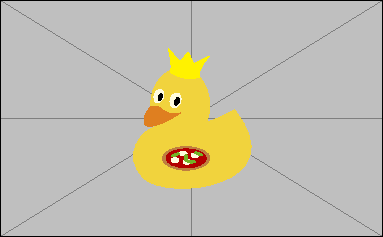
\includegraphics[width=\textwidth]{images/example-image-duck}
    \caption{One figure or several subfigures of the different lanes}
    \label{fig:impl-environment-lanes}
\end{figure}

\todo{Glemte, hvad jeg mere ville skrive, men der skal i hvert fald lidt beskrivelse af banerne og hvilke er træningsbaner vs testbane}
